\documentclass[a4paper,12pt]{report}
\usepackage[utf8]{inputenc}
\usepackage[T1]{fontenc}
\usepackage[english]{babel}
\usepackage{lmodern}

%Figure progressive enumeration
\usepackage{chngcntr}
\counterwithin{figure}{chapter}
\counterwithin{table}{chapter}

%package used to enumerate figures
\usepackage[labelfont=bf]{caption}

%hyperref for interactive PDF index
\usepackage[bookmarks, colorlinks, breaklinks]{hyperref}
\hypersetup{linkcolor=black, citecolor=black, filecolor=black, urlcolor=black}

%Package required to use special symbols
\usepackage{amsmath, amssymb}

%Package required to use figures
\usepackage{graphicx}
%Include the bibliography in the table of contents
\usepackage{tocbibind}

%Package used to insert figures at the specified position
\usepackage{float}

%Our chapters must be called sections
\addto\captionsenglish{\renewcommand{\chaptername}{Section}}

\begin{document}

%Code for title page
\begin{titlepage}
\centering
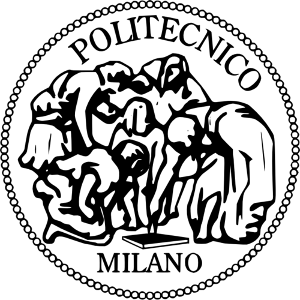
\includegraphics[width=0.20\textwidth]{./pictures/logo_poli}\par
	\vspace{1.5cm}
	{\Large {PowerEnJoy \\ 
		Software Engineering II} \par}
	\vspace{1.5cm}
	{\LARGE \textbf{Integration Test Plan Document} \par}
	\vspace{1.5cm}
	{\Large\itshape Giovanni Scotti, Marco Trabucchi\par}
	\vspace{2cm}
	\vfill
	% Bottom of the page
	{\large Document version: 1\par}
	{\large \today \par}
\end{titlepage}

%Make the table of contents
\tableofcontents

%INTRODUCTION
\chapter{Introduction}
\label{ch:Introduction}

\section{Purpose and Scope}
\subsection{Purpose}
The Integration Test Plan Document (ITPD) is intended to provide the guidelines to accomplish the integration test phase planning in sufficient detail. This also includes determining which tools are needed and will be used during the testing process itself, as well as the required stubs, drivers and data structures that will be useful during said process.

\subsection{Scope}
PowerEnJoy is a car sharing service that only employs electric vehicles; it is provided for a large city, and aims to support the sharing process and car management of the electric cars, as well as the booking and payments for the service itself.

\section{Definitions, Acronyms, Abbreviations}
\begin{description}
\item[RASD:] Requirements Analysis and Specification Document.
\item[System:] The software system-to-be, in all of its entirety.
\item[Driver:] See \textbf{User}.
\item[User:] Any person subscribed to the service who rents a car using \hbox{\emph{PowerEnJoy}}.
\end{description}



\section{Reference Documents}
This document follows the guidelines provided by ISO/IEC/IEEE 1016:2009~\cite{ieee-1016} related to system design and software design descriptions for complex software systems.

The indications provided in this document are also based on the ones stated in the previous deliverable for the project, the RASD document~\cite{rasd}.

Moreover it is strictly based on the specifications concerning the RASD assignment~\cite{se-assignments} for the Software Engineering II project, part of the course held by professors Luca Mottola and Elisabetta Di Nitto at the Politecnico di Milano, A.Y. 2016/17.

\chapter{Integration Strategy}

\section{Entry Criteria}
This section expresses the prerequisites needed to be met before the integration phase takes place.

\begin{description}
\item[Documentation:] The documentation for every method and class must be provided for each individual component, in order to make it easier to reuse classes and understand their functioning; this is in fact also a prerequisite for the unit tests to be performed before the integration test phase. When necessary, a formal language specification of the classes' behaviours can be used (such as JML - Java Modelling Language).
\item[Unit tests:] All the classes and methods must be tested thoroughly using JUnit, in order to assure a properly correct behaviour of the internal mechanics of the individual components. It is required that the test coverage of each class and package reaches 90\% of the code lines; moreover, test cases must be written with continuity and executed at every consecutive build of the project: this is needed in order to ensure that newly added lines do not interfere with the stability of the rest of the code.
\item[Code Inspection and Analysis:] Both automated data-flow analysis and code inspection must be performed on the whole project classes. This will reduce the risk that, during the integration test phase, any code-related issues or bugs rise, leading to more complex problematic situations to be solved in latter phases of the project development, with much greater effort for the development team.
\item[RASD and DD:] Along with the indications provided in this very document (ITPD), the two previous documents for this project, RASD and DD, must be delivered before the integration test phase can begin.
\end{description}

\section{Elements to be Integrated}

\section{Integration Testing Strategy}

\section{Sequence of Components/Function Integration}

\chapter{Individual Steps and Test Description}

\chapter{Tools and Test Equipment Required}

\chapter{Program Stubs and Test Data Required}

\appendix
\chapter{Appendix}
\section{Software and tools used}
\begin{itemize}
\item \LaTeX, used as typesetting system to build this document.
\item draw.io - \url{https://www.draw.io} - used to draw diagrams and mock-ups.
\item GitHub - \url{https://github.com} - used to manage the different versions of the document and to make the distributed work much easier.
\item GitHub Desktop, the GitHub official application that offers a seamless way to contribute to projects.
\end{itemize}
\section{Hours of work}
The absolute major part of the document was produced in group work. The approximate number of hours of work for each member of the group is the following:

\begin{itemize}
\item Giovanni Scotti: 25 hours
\item Marco Trabucchi: 20 hours
\end{itemize}

NOTE: indicated hours include the time spent in group work.

\begin{thebibliography}{1}

\bibitem{ieee-29148}
	ISO/IEC/IEEE 29148:2011 \emph{Systems and software engineering - Life cycle processes - Requirements engineering}
	
\bibitem{se-assignments}
	AA 2016/2017 Software Engineering 2 - \emph{Project goal, schedule and rules}

\end{thebibliography}

\end{document}